\documentclass{article}
\usepackage[utf8]{inputenc}
\usepackage{mathtools}
\usepackage{amssymb}
\usepackage{graphicx}
\usepackage{listings}
\usepackage{float}
\usepackage{gensymb}
\usepackage{amsthm}
\usepackage{longtable}
\usepackage{adjustbox}
\usepackage{physics}

\theoremstyle{definition}
\newtheorem{definition}{Definition}
\newtheorem{proposition}{Proposition}
\newtheorem{theorem}{Theorem}
\newtheorem{corollary}{Corollary}
\newtheorem{lemma}{Lemma}
\newtheorem{example}{Example}
\newtheorem{claim}{Claim}

\title{Differential Geometry}
\author{quinten tupker}
\date{October 8 2020 - \today}

\begin{document}

\maketitle

\section*{Introduction}

These notes are based on the course lectured by Dr Jack E Smith in Michaelmas
2020. Due to the measures taken in the UK to limit the spread of
Covid-19, these lectures were delivered online. These are not meant to be an
accurate representation of what was lectures. They solely represent a mix of
what I thought was the most important part of the course, mixed in with many
(many) personal remarks, comments and digressions... Of course, any
corrections/comments are appreciated.

Unlike some of the other courses, there is no real introduction here, and we
jump straight into the content!

\section{Manifolds and Smooth Maps}

Manifolds are spaces that locally look like $\mathbb{R}^n$. Formally this is:

\begin{definition}
  $X$ is a \textbf{topological $n$ manifold} if $X$ is a second countable
  Hausdorff topological space such that $\forall p \in X \exists \text{open} U
  \ni p$ and open $V \subseteq \mathbb{R}^n$ and homeomorphism $\phi : U \to V$.
\end{definition}

Here,

\begin{definition}
  Topological space $X$ is \textbf{Hausdorff} if for every distinct $x, y \in X$ there
  exists open $U \ni x, V \ni y$ in $X$ such that $U \cap V = \emptyset$.
\end{definition}

and

\begin{definition}
  Topological space $X$ is \textbf{second countable} if there exists a set of
  open sets $\mathcal{U}$ st that every open set in $X$ can be written as a
  union of sets in $\mathcal{U}$
\end{definition}

Since these two properties transfer to subsets, any subset of a topological $n$
manifold is also a topological $n$ manifold. Also, to give some more intuition,
the condition that $X$ is a seond countable Hausdorff topological space is
exactly equivalent to the condition that $X$ is metrizable and has countably
many components. It is just tradition that it is defined as above. Some more
defintions. Above, $\phi$ is called the \textbf{chart}, $U$ is called the
\textbf{coordinate patch}, although in some cases can also be called the chart.
The functions $x_1 \circ \phi, \dots, x_n \circ \phi$ (so the components of
the result) are called the \textbf{local coordinates}, and $\phi^{-1}$ is called
the \textbf{paramaterisation}, although that term is not used that frequently.
Finally, for overlapping charts, we can define the \textbf{transition map}
between them as $\phi_2 \circ \phi_1^{-1} : \phi_1 (U_1 \cap U_2) \to \phi_2(U_1
\cap U_2)$.

Now, we want to generalise calculus to manifolds, so it makes sense to start by
trying to generalise the notion of smoothness. The simplest approach would be to
say that $f$ is smooth on $X$ if it is smooth on the local coordinates. The
issue then arises that this may not be consistent with smoothness on other
charts (where these overlap). As such, we need to require that the transition
maps are smooth as well. Consequently we do the following:

\begin{definition}
  The \textbf{atlas} of a manifold is a collection of charts of a topological
  n manifold that covers all of $X$.
\end{definition}

An atlas is \textbf{smooth} if all transition maps are smooth, and a map $f$ is
\textbf{smooth} on atlas $\mathfrak{A}$ if $f \circ \phi_\alpha^{-1}$ is smooth
$\forall \alpha$. As a result all local coordinate functions are smooth. Now,
really, specifying the atlas precisely all the time is somewhat tedious, and
somehow not the point, so we want a degree of flexibility. For this we define

\begin{definition}
  Two atlases are \textbf{smoothly equivalent} if their union is smooth.
\end{definition}

Note that this forms an equivalence relation (apply the chain rule on transition
functions for transitivity).

\begin{definition}
  A \textbf{smooth structure} is an equivalence class of atlases.
\end{definition}

As we hope, we do indeed have that if a function is smooth wrt to an atlas, it
is smooth wrt to any atlas in its smooth structure. Also, we can define a
maximal atlas to be the union of all the atlases in a smooth structure, if we
deem that to be convenient (includes trivial changes like translating or scaling
the local coordinates).

\begin{definition}
  A \textbf{smooth $n$ manifold} is a topological $n$ manifold with a smooth
  structure.
\end{definition}

Note that under the product topology, the product of two manifolds naturally
forms a new (smooth) manifold. Also, a remarkable fact is that for $n=1, 2, 3$
all topological $n$ manifolds have an essentially unique smooth structure,
whereas this breaks down for $n \geq 4$. Also, a new chart is said to be
\textbf{compatible} with an atlas if when added to the atlas, the atlas remains
smooth.

Finally, to give a concrete example of a manifold, we may consider $S^n$, which
forms a manifold with two charts: one being the sphere without the North pole,
and the other being the sphere without the South pole, $U_\pm$ with charts

$$ \phi_\pm(y_0, \dots, y_n) = \frac{1}{1 \mp y_0} (y_1, \dots, y_n), $$

where the local coordinates are referred to as $x^\pm$. [End of DG1]

\subsection{Forming Manifolds from Sets (Instead of Topological Spaces)}

We observe that an atlas can generate a topology. In particular if we consider
the data

\begin{itemize}
\item set $X$
\item subsets $U_\alpha \subseteq X$
\item open sets $V_\alpha \subseteq \mathbb{R}^n$
\item bijections $\phi_\alpha : U_\alpha \to V_\alpha$ that have smooth
  transition functions, and $\forall \alpha, \beta, \phi_\alpha(U_\alpha \cap
  U_\beta)$ is open in $V_\alpha$ (weird but useful)
\end{itemize}

then we see that if we declare $U$ to be open iff $\phi_\alpha(U \cap U_\alpha)$
is open $\forall \alpha$, then this forms a topology (easy) and 

\begin{proposition}
  Apart from the possible failure of Hausdorff and second countable, using the
  above data as specified turns $X$ into a topological $n$ manifold, and
  $\{\phi_\alpha\}$ into a smooth atlas (so we have a smooth manifold).
\end{proposition}

\begin{proof}
  It suffices to show that $U_\alpha$ are open and that $\phi_\alpha$ are
  homeomorphisms (smoothness follows from the smoothness of the transition
  functions). As such it is sufficient to show that some $U \subseteq U_\alpha$
  is open iff $\phi_\alpha(U)$ is open in $V_\alpha$ (this is to show that
  $\phi_\alpha$ is a homeomorphism, which implies taht $U_\alpha$ is open by the
  openness of $V_\alpha$). One direction is clear: if $U$ is open, then by
  declaration, $\phi(U \cap U_\alpha = U)$ is open. Conversely, if $\phi(U)$ is
  open then we want that $\forall \beta, \phi_\beta(U \cap U_\beta)$ is open,
  but we observe that
  \begin{align*}
    \phi_\beta(U \cap U_\beta)
    &= \phi_\beta \circ \phi_\alpha^{-1} (\phi_\alpha(U \cap U_\beta)) \\
    &= (\phi_\alpha \circ \phi_\beta^{-1})^{-1}
      (\phi_\alpha(U) \cap \phi_\alpha(U_\alpha \cap U_\beta))
  \end{align*}
  Here $\phi_\alpha(U_\alpha \cap U_\beta)$ is open as an intersection of
  $V_\alpha \cap V_\beta$, and $\phi_\alpha(W)$ is open by assumption. The
  transition function is continuous by assumption. So done. 
\end{proof}

Finally, we note that we can define this set of $\phi$s and $U$s and $V$s, etc.
to be a ``pseudo-chart'', and can define a ``smooth pseudo-structure,'' etc.
from here. All we really want to show is that the toplogy is secondary once we
have a good set of functions. In fact, using this approach we can skip $X$
entirely, and start from sets $U_\alpha$ that we identify with different real
spaces, and then stitch together with arbitrary pseudo-charts. That can
definitely be done, but generally is quite complicated with many more moving
parts, and so we usually, at least for the purpose of a course, start with a
structure in mind, and turn that into a manifold, instead of stitching an
arbitrary one together (although that may be a good source of counter examples).

Unfortunately, it does remain the case that showing Hausdorff and
second-countable is still hard, although there are some tricks to do so. For
second countability, using the subset of all rational balls will always work if
the number of charts is countable. For Hausdorffness, as long as two points live
in the same chart, we are immediately done, so combining charts and considering
the exceptions can be an efficient approach.

\subsection{Projective Spaces and Grassmannians}

Today we do an extended example to develop some more interesting manifolds.
First, we look at the real projective linear space $\mathbb{RP}^n,$ which is the
space $\mathbb{R}^{n + 1} \setminus \{0\}$ under the equivalence relation $x \sim y$ iff
$\exists \lambda \in \mathbb{R} \setminus \{0\}, x = \lambda y$. As such, any
point can be labelled by the \textit{ratio} of coordinates $[x_0 : x_1 : \dots :
x_n]$, and for the purpose of comparison, we are free to set any nonzero
coordinate $x_i$ to 1.

To turn this into a smooth $n$-manifold, let's consider the following
pseudo-chart:

\begin{align*}
  U_i &= \{[x_0 : x_1 : \dots : x_n] | x_i \neq 0\} \\
  \phi_i([x_0 : x_1 : \dots : x_n]) &= \frac{1}{x_i} (x_0, \dots, \hat{x_i}, \dots, x_n)
\end{align*}

where $\hat{x_i}$ means omit $x_i$ from the list. 

\begin{lemma}
  These form a pseudo-atlas.
\end{lemma}
\begin{proof}
  Need to show $\phi_i(U_i \cap U_j)$ open and $\phi_j \circ \phi_i^{-1}$
  smooth. wlog, $i=0, j=1$ and $s, t$ are our local coordinates of interest.
  With a little thought we see $\phi_0(U_0 \cap U_1) = \{s_1 \neq 0\}$ which is
  open. To see $\phi_1 \circ \phi_0^{-1}$ is smooth, notice that
  \begin{align*}
    \phi_0^{-1}(s) &= [1 : s_1 : \dots : s_n] \\
    \phi_1^{-1}(t) &= [t_1 : 1 : \dots : t_n]
  \end{align*}
  and consequently we see that certainly
  $$ \phi_1 \circ \phi_0^{-1}(s) = \frac{1}{s_1}[1 : s_1 : \dots : s_n] $$
  is smooth, so indeed we have pseudo-atlas.
\end{proof}

All that is left now is to show that $\mathbb{RP}^n$ is second countable and
Hausdorff. Second countability follows from the finite number of covers that we
are using. Hausdorffness is harder though. We cannot use our previous tactic of
relying on the fact that any two points will lie in at least some chart. So
instead we expand our atlas until that is the case. Above, we essentially formed
charts using the standard unit vector basis, and omitted that each time. This
can be generalised in two ways. Firstly, we can expand to any basis, which
copies the above approach and is entirely straight forward. Secondly, we can
consider a space $W$ to be our line in $\mathbb{R}^n$, and any complement $W'$
of it. This abstracts the notion, but it has its uses as well.

Taking this approach, we see that for a given line input $T$ the projection
$\pi_W |_T$ restricted to $T$ is a bijection (as these have forcibly the same
dimension) so taking

$$ \psi_T = \pi_W' \circ (\pi_W |_T)^{-1} : W \to W' $$

allows us to biject from our manifold to $W'$ which is isomorphic to
$\mathbb{R}^n$, giving us a chart. It is an exercise on the example sheet to
show this is compatible. Consequently, filling these all, we can show that the
space is Hausdorff as well, meaning that $\mathbb{RP}^n$ forms a smooth
$n$-manifold. Now, just as a note, really, we are not identifying the line $T$
with a point in $W'$. Rather, we are identifying $T$ with the map $\psi_T$. This
will be relevant.

Now, one generalisation we will make, is to that of the \textbf{Grassmannian}.
The Grassmannian, $Gr(k, n)$ is thespace of $k$-subspaces within $\mathbb{R}^n$.
Note in particular that $\mathbb{RP}^n = Gr(1, n + 1)$. And since we identify
subspaces $T$ with $\psi_T$ we also see that $\text{dim} Gr(k, n) = \text{dim}
\mathcal{L}(W, W') = k(n - k)$. Finally, we want to remark that we can use
$\mathbb{C}$ instead of $\mathbb{R}$, to give use $\mathbb{CP}^n$, and
$Gr_{\mathbb{C}}(k, n)$. Incidentally, the transition maps here are not only
smooth, but also holomorphic, meaning that these form complex manifolds. [End of
DG 3]

\subsection{Smoothness of Maps Between Manifolds}

So how do we define the smoothness of a map between manifolds (instead of to a
Euclidean space)? As expected, we just work with local coordinates. Consequently
for smooth manifolds $X, Y$ of respective dimension $n, m$ with respective
atlases $\phi_\alpha : U_\alpha \to V_\alpha, \psi_\beta : S_\beta \to T_\beta$,
then 

\begin{definition}
$F: X \to Y$ is \textbf{smooth} wrt to these atleses iff $\forall \alpha, \beta$

$$ \psi_\beta \circ F \circ \phi_\alpha^{-1} : \phi_\alpha(F^{-1}(S_\beta)) \to
T_\beta $$

is smooth as a map between open subsets in $\mathbb{R}^n$ and $\mathbb{R}^m$.
Importantly, this definition only makes sense if $F$ is \textbf{continuous}, and
in particular we require $F^{-1}(S_\beta)$ to be open for this definition to
make sense.
\end{definition}

From here, we remark some trivial lemmas [which I won't write up properly] that
due to the smoothness of transition functions, it suffices to check that $F$ is
smooth in the neighbourhood of some point of a single chart. If that holds for
all points, then $F$ is smooth as well. We also see that smoothness depends only
on the smooth structure, and not the precise atlas, as one may expect.

Finally, again some more sanity check lemmas. It is easy to see that this
definition coincides with the usual definition of smoothness between finite
dimesinonal real spaces, and also corresponds to the definition of smoothness
from a manifold to $\mathbb{R}$ used earlier in this course. More importantly,
we also see that a composition of smooth maps as smooth, and finally, this is
one result I will write down as a lemma, we see that smoothness is a local
property of the map:

\begin{lemma}
Smoothness is \textbf{local in source}, meaning $\forall F: X \to Y$, $F$ is
smooth iff $\exists \text{open cover} W_\gamma$ st $\forall \gamma, F
|_{W_\gamma}$ is smooth.
\end{lemma}

This is indeed a neat way of saying that a property is truly local in nature. 

In line with our previous approach, we'd like to be able to specify smoothness
without relying on the topology of the space. It is a bit pedantical, but
nevertheless here we go:

\begin{proposition}
$F: X \to Y$ is smooth iff $\exists$ cover (not necessarily smooth - we
  can't rely on the topology) $W_{\gamma \in \mathcal{C}}$ of $X$ st $\forall
  \gamma \exists \alpha(\gamma) \in \mathcal{A}, \beta(\gamma) \in \mathcal{B}$
  such that:
\begin{enumerate}
  \item $W_\gamma \subseteq U_{\alpha(\gamma)}$ and $F(W_\gamma) \subseteq
    S_{\beta(\gamma)}$
  \item $\phi_{\alpha(\gamma)}(W_\gamma)$ open in $V_{\alpha(\gamma)}$
    (equivalent to saying $W_\gamma$ open in $X$ once the topology has been
    enforced)
  \item $\psi_{\beta(\gamma)} \circ F \circ \phi_{\alpha(\gamma)} |_{W_\gamma}$
    is smooth.
  \end{enumerate}
\end{proposition}
\begin{proof}
\begin{itemize}
\item only if: pick $\mathcal{C} = \mathcal{A} \times \mathcal{B}$, and
  $\alpha, \beta$ as projection maps, and $W_\gamma = U_{\alpha} \cap
  F^{-1}(S_\beta )$. Then the result follows.
\item if: we only need to check that $F$ is cont, so that $F^{-1}(S)$ is open
  for open $S$, or equivalently, since we know the $W_\gamma$ will turn out to
  be open, that $F^{-1}(S) \cap W_\gamma$ is open each time. To do so we note
  that $\phi_\alpha$ is a homeomorphism, we we're done if the following is open:
  \begin{align*}
    \phi_\alpha(F^{-1}(S) \cap W_\gamma)
    &= \phi_\alpha(F^{-1}(S \cap S_\beta) \cap W_\gamma) \\
    &= \phi_\alpha(F^{-1}(S \cap S_\beta)) \cap \phi_\alpha(W_\gamma) \\
    &= (\psi_\beta \circ F \circ \phi_\alpha^{-1})^{-1} (\psi_\beta(S)) \cap \phi_\alpha(W_\gamma)
  \end{align*}
  which is certainly open.
\end{itemize}
\end{proof}

\begin{example}
  $H : S^{2n + 1} \to \mathbb{CP}^n$, the Hopf map, is an example of a smooth
  map.
\end{example}

Finally, we'd like to define some notion of equivalence on manifolds. Here we
define

\begin{definition}
  A \textbf{diffeomorphism} is a smooth invertible map between manifolds with a
  smooth inverse.
\end{definition}

\begin{definition}
  Two manifolds are diffeomorphic when there exists a diffeomorphism between
  them.
\end{definition}

You might think that since we're doing geometry, and not topology, we care about
the values involved, and these equivalence classes are not of interest, but
really, these equivalence classes have less to do with the space, and more to do
with the smooth structure on them. If you change charts, then you also may have
to change the functions involved. As such, diffeomorphism establish an
equivalence between smooth structures more than between manifolds. This is
particularly relevant for the time, as before, when we said that for $n \leq 3$
all manifolds have an essentially unique smooth structure. Here ``essentially
unique'' meant unique up to diffeomorphism.

\begin{example}
  A particularly famous manifold is the Riemann sphere, which is in this context
  often defined to be $\mathbb{CP}^1$, but is diffeomorphic to $S^2$, and
  $\mathbb{C} \cup \{\infty\}$ via either the stereographic projection or
  identifying via normalising (normalise $[z_0 : z_1]$ to $[1 : z]$ or
  ``$\infty$'' for $\mathbb{C} \cup \{\infty\}$, etc.).
\end{example}

Finally, we do have a somewhat important result that comes out from here:

\begin{lemma}
  If smooth manifolds $X, Y$ are diffeomorphic, then they are of the same
  dimension.
\end{lemma}
\begin{proof}
  Fix diffeomorphism $F: X \to Y, p \in X, U \ni p, V \ni F(p), \phi : U \to V,
  \psi : S \to T$ such that $U, V, S, T$ open and shrink them such that $F(U) =
  S$, then let $G = \psi \circ F \circ \phi^{-1}$, $H = \phi \circ F^{-1} \circ
  \phi^{-1}$, then both of these are differentiable, and mutually inverse maps
  on subsets of $\mathbb{R}^n, \mathbb{R}^m$. Taking derivatives we get two
  linear maps that are mutually inverse, and so must be of the same dimension,
  meaning $m = n$.
\end{proof}
[End of DG 4]

\subsection{Tanget Spaces}

We want to define tangent spaces on abstract manifolds.

\begin{definition}
  A \textbf{curve based at $p$} is a curve, $\gamma : I \to X$ where $I$ is an
  open subset of $\mathbb{R}$ such that $\gamma(0) = p$. (they also have to be
  somewhat smooth)
\end{definition}

\begin{definition}
  Two curves $\gamma_1, \gamma_2$ based at $p$ \textbf{agree to first order} iff
  $\exists$ a chart such that
  $$ (\phi \circ \gamma_1)'(0) = (\phi \circ \gamma_2)'(0) $$
\end{definition}

This forms an equivalence relation. Reflexivity, and symmetry are clear,
however, transitivity is not entirely obvious. Hence we have the lemma

\begin{lemma}
  If two curves agree to first order according to one chart, they agree to first
  order according to any chart.
\end{lemma}
\begin{proof}
  Just apply the chain rule to the transition functions.
\end{proof}

As such we then say

\begin{definition}
  The \textbf{tangent space} of $X$ at $p$, $T_pX$ is the set of curves at $p$
  modulo agreement to first order. Elements of this set are denoted $[\gamma]$
  (for the equivalence class).
\end{definition}

Now, if we define the map

\begin{align*}
  \pi^\phi_p : \{ \text{curves based at } p\} &\to \mathbb{R}^n \\
  \gamma &\mapsto (\phi \circ \gamma)'(0)
\end{align*}

then we see that modulo agreement to first order this is injective. Furthermore,
if we show it surjective, we so $T_pX$ is isomorphic to $\mathbb{R}^n$:

\begin{proposition}
  $T_pX$ is isomorphic to $\mathbb{R}^n$ and $\pi^\phi_p$ is an isomorphism.
\end{proposition}
\begin{proof}
  We just need to show $\pi_p^\phi$ is surjective. $\forall v \in \mathbb{R}^n$
  consider $\gamma(t) = \phi^{-1} (\phi(p) + tv)$. This works.
\end{proof}

Now, as a matter of notation we use $\partial_i$ or $\partial_{x_i}$ to denote
$(\pi^\phi_p)^{-1}(e_i)$. Clearly, this notation has connotations, but
interestingly these turn out to be well-founded, for the following two reasons:

\begin{proposition}
  Vectors transform as
  $$ \partial_{y_i} = \sum_j \partial_{y_i} x_j \partial_{x_j} $$
\end{proposition}
\begin{proof}
  \begin{align*}
    \partial_{y_i} &= (\pi^{\phi_2}_p)^{-1}(e_j) \\
    &= (\pi^{\phi_1}_p)^{-1} (\sum_j \partial_{y_i} x_j e_j) \\
    &= \sum_j \partial_{y_i} x_j (\pi^{\phi_1}_p)^{-1} (e_j) \\
    &= \sum_j \partial_{y_i} x_j \partial_{x_j}
  \end{align*}
\end{proof}

Furthermore, we can see that when written in the standard unit basis
$\partial_i$, any $[\gamma]$ has its coefficients precisely the values it gets
as its derivatives, so one can interpret these vectors as derivatives to a
certain extent. [End of DG 5]

\subsection{Vectors as Differential Operators}

In the last section, we discussed a geometric way to derive and think about
tangent vectors. However, we can also do so in an algebraic manner. That is what
we do here.

If we are to describe tangent vectors algebraically as differential operators,
then we want to describe them as ``hitting'' something. What will they hit,
well, quite naturally, they will hit functions from the manifold. Consequently,
we consider a function $f : U \to \mathbb{R}$ for open $U \ni p$ for some point
$p$, and then the result of the hitting along some path would be $(f \circ
\gamma)'(0)$ (so we are interested in what this ``hitter'' may be).

But we also want to relate this to our original picture of vectors, so we have:

\begin{lemma}
  $(f \circ \gamma)'(0)$ depends only on $[\gamma]$, and for $[\gamma] = \sum
  a_i \partial_i$, we have
  $$ (f \circ \gamma)'(0) = \sum a_i \partial_i f |_p $$
\end{lemma}
\begin{proof}
\begin{align*}
(f \circ \gamma)'(0) 
&= \frac{d}{dt} |_{t=0} ((f \circ \phi^{-1}) \circ (\phi \circ \gamma))(t) \\
&= \sum_i \partial_{x_i} f |_p (x_i \circ \gamma)'(0)
\end{align*}
since $f \circ \phi^{-1}$ is just $f$ written in terms of the local coordinates. 
\end{proof}

So we see that combined with a hitter, we can turn any $\gamma$ into a
differential operator on $f$, but we can make a further simplification. We
notice in particular that we don't really care that much about the open
neighbourhood $U$ containing $p$. As such we define

\begin{definition}
The \textbf{germ} of smooth $f$ at $p$ is the equivalence class $[(U, f)]$ for
smooth $f: U \to \mathbb{R}$, open $U \ni p$ modulo the equivalence relation
$(U_1, f_1) \sim (U_2, f_2)$ iff there exists open $V \ni p$ such that $V
\subseteq U_1, U_2$, and $f_1 |_V = f_2 |_V$.
\end{definition}

We call the space of germs at $p$, $\mathcal{O}_{X, p}$. Now we add some
algebraic definitions that, as far as I can tell, serve little purpose in this
context: note that by using constant functinos we can easily construct a
homomorphism $\mathbb{R} \to \mathcal{O}_{X, p}$. turning it into an
$\mathbb{R}$-algebra. Also,

\begin{lemma}
As a ring (which it forms), $\mathcal{O}_{X, p}$ has
a unique maximal ideal $\mathfrak{m}$ which is precisely the set of functions
that vanish at $p$. 
\end{lemma}
\begin{proof}
$\mathfrak{m}$ forms a maximal ideal since it is the kernel of a homomorphism to
a field: $[(U, f)] \mapsto f(p)$. It is unique, since for any element outside of
this ideal, choosing $U$ to be small, we can see $f$ is always nonzero, meaning
that the ring contains a multiplicative inverse of our element $[(U, 1/f)]$, but
if an ideal contains an invertible element, that ideal is the whole ring, and so
$\mathfrak{m}$ is the unique maximal ideal.
\end{proof}

Precisely because of the situation that occurs here, rings with a unique maximal
ideal are called \textbf{local} rings. Even in other context, one still imagines
that maximal ideal as being the place where some function vanishes. 

Having worked so far (although the algebra bit still seems unnecessary to me),
we see that we can hit functions with vectors to get real numbers via

$$ T_pX \times \mathcal{O}_{X, p} \to \mathbb{R} $$

or equivalently there exists 

$$ D: T_PX \to \mathcal{O}^\vee_{X, p} $$

where $\mathcal{O}^\vee_{X, p}$ is the dual of $\mathcal{O}_{X, p}$, ie. $D$
converts vectors into hitters of functions (so as originally described,
combining a vector $v$ with something $D$ allows us to hit functions). Now,
really, we hope that somehow $D$ forms an isomorphism. Certainly $D$ is well
defined (will see), and injective (see how it transforms the unit basis vectors
$\partial_i$), but we see it is not surjective. However, on closer observation,
we see that $D$ maps only to a very small subset of $\mathcal{O}^\vee_{X, p}$.
In particular, it maps to a subset satisfying the property

\begin{lemma}
$$ D(v)(fg) = D(v)(f) g(p) + f(p) D(v)(g) $$
\end{lemma}
\begin{proof}
Apply the chain rule to $(fg) \circ \gamma$.
\end{proof}

As such, we make the following (far too general for this context) definition:

\begin{definition}
For ring $R$, $R$-algebra $S$, and $S$-module $M$, an $R$-linear
\textbf{derivation} from $S$ to $M$ is an $R$-linear map $d: S \to M$ satisfying 
$$ d(fg) = d(f)g + fd(g) $$
The set of derivations is denoted by $\text{Der}_R(S, M)$, which is a submodule
of $\text{Hom}_R(S, M)$.
\end{definition}

I mean, this is clearly just an algebraic definition of something like a first
order differential operator. We would also like to note that $d(r) = 0 \forall r
\in R$, since $d(r) = rd(1)$ and $d(1) = d(1) + d(1) = 2d(1)$ so $d(1) = 0$.

Now certainly, $D(v) \in \text{Der}_\mathbb{R}(\mathcal{O}_{X, p}, \mathbb{R})$
where the relevant bits form $\mathbb{R}$ algebras once we consider constant
functions. Of course, the whole point of this otherwise random introduction of
derivations is that we get an isomorphism:

\begin{proposition}
$D : T_pX \to \text{Der}_\mathbb{R}(\mathcal{O}_{X, p}, \mathbb{R})$ is an isomorphism.
\end{proposition}
\begin{proof}
Certainly $D$ is linear and injective. Then it remains for us to show that $D$
is surjective. In order to do so we pick any derivation $\delta$ and want to
show $\exists v, D(v) = \delta$. To do so we consider something like the Taylor
series of $f$ for any $[U, f] \in \mathcal{O}_{X, p}$. If we then pick local
coordinates such that $x(p) = 0$, then we see that all constant terms in the
series are eliminated ($d(\text{const}) = 0$), and quadratic terms and higher
are eliminated as well, leaving us with
$$ \delta(f) = \delta(\sum_i x_i \partial_{x_i}f|_p) = \sum_i \delta(x_i)
D(\partial_{x_i})(f)$$
From here we see clearly that 
$$ v = \sum_i \delta(x_i) \partial_{x_i} $$
does the trick. That's all fine and well, but the above formula depends on the
existence of a kind of Taylor series. To find something like that we consider
the following. For any germ $[(U, f)]$, consider $g: U \to \mathbb{R}$ given by
$$ g =
\begin{cases}
\frac{f(x_1, \dots, x_n) - f(x_1, \dots, x_{n-1}, 0)}{x_n} & x_n \neq 0 \\
\partial_{x_n} f & x_n = 0
\end{cases}
$$
then by l'Hopital's rule, this is continuous. Now define
$f_n(x_1, \dots, x_n) = f(x_1, \dots, x_{n - 1}, 0)$, then we get first order
pseudo-Taylor series
$$ f = f_n + x_n g $$
with property
$$ \delta(f) = \delta(f_n) + \delta(x_n) g(p) + x_n(p) \delta(g) = \delta(f_n)
+ \delta(x_n) \partial_{x_n} f|_p$$
which once we apply it to each coordinate completes our proof.
\end{proof}

[End of DG 6]

\subsection{Derivatives of Smooth Maps}

The natural next step is to find a way to express derivatives on maps between
smooth manifolds. That is, to find linear approximations. Since the spaces
themselves aren't linear, the only plausible way to implement any kind of linear
map is to consider a linear map between the tangent spaces $T_pX \to T_{F(p)}Y$
for $F: X \to Y$. As such we define

\begin{definition}
The \textbf{derivative} of $F$ at $p$ is the map $D_pF : T_pX \to T_{F(p)}Y$
given by $[\gamma] \mapsto [F \circ \gamma]$. This map may also be denoted by
$F_*$ the pushforward by $F$ on tangent vector spaces.
\end{definition}

\begin{lemma}
This is well defined and linear, and
$$ D_pF(\partial_{x_i}) = \sum_j \partial_{x_i} y_j|_p \partial_{y_j} $$
\end{lemma}
\begin{proof}
Linearity and well-definedness can be checked easily. What remains is for us to
check the formula. As such,
$$ \frac{d}{dt} |_p (y_j \circ F \circ \phi^{-1}) (\phi(p) + te_i) =
\partial_{x_i} y_j $$
as required.
\end{proof}

We note that this coincides with the standard multivariate calculus definition
of the derivative. Also, we notice that any vector $[\gamma]$ can be written as
$D_0 \gamma(\partial_t) = [\gamma]$. Furthermore, the chain rule follows
straight from this definition as
\begin{proposition}
The \textbf{chain rule} states that
$$ D_p(G \circ F) = D_{F(p)}G \circ D_p F $$
\end{proposition}
\begin{proof}
$$ D_p(G \circ F)([\gamma]) = [G \circ F \circ \gamma] = D_{F(p)}G \circ
D_pF([\gamma]) $$
\end{proof}

That finishes the main topic for this section, the definition of the derivative,
but for completeness, we will include how one may define the derivative from the
algebraic point of view of derivations. As a side note, since it may not be
clear what the purpose of the algebraic perspective is. I hear this is the
primary focus in Algebraic Geometry. Anyhow, moving on

That finishes the main topic for this section, the definition of the derivative,
but for completeness, we will include how one may define the derivative from the
algebraic point of view of derivations. As a side note, since it may not be
clear what the purpose of the algebraic perspective is. I hear this is the
primary focus in Algebraic Geometry. Anyhow, moving on. As such we define

\begin{definition}
The \textbf{pullback}, $F^*$ by $F$ from $\mathcal{O}_{Y, F(p)}$ to $\mathcal{O}_{X,
  p}$ mapping $[(U, f)]$ to $[(F^{-1} (U), f \circ F)]$.
\end{definition}

This is well defined, and since it is $\mathbb{R}$-linear we have dual map

$$ (F^*)^\vee : \mathcal{O}^\vee_{X, p} \to \mathcal{O}^\vee_{Y, F(p)} $$.

but really, one may observe that these maps preserves the spaces we want it to
preserve. Namely, it restricts nicely to a map

$$ (F^*)^\vee : \text{Der}_\mathbb{R}(\mathcal{O}_{X, p}, \mathbb{R}) \to
\text{Der}_\mathbb{R}(\mathcal{O}_{Y, F(p)}, \mathbb{R}) $$

but of course, since these are equivalent to tangent spaces, this is just
another way of implementing the derivative. 

\begin{lemma}
The appropriate diagram commutes, meaning that $D \circ D_pF = (F^*)^\vee \circ D$.
\end{lemma}
\begin{proof}
$\forall [\gamma] \in T_pX, f \in \mathcal{O}_{Y, F(p)}$ it holds that
\begin{align*}
D(D_pF([\gamma]))(f) 
&= D([F \circ \gamma])(f) \\
&= (f \circ F \circ \gamma)'(0) \\
&= D([\gamma])(F^*f) \\
&= (F^*)^\vee (D([\gamma]))(f)
\end{align*}
\end{proof}

So we now have two parallel ways to define the derivative. In different
situations, a different approach will be more useful than the other. Overall, a
lot of notation and terms are used, but fundamentally, the concepts we've seen
so far are nothing unsurprising. [End of DG 7]

\subsection{Immersions, Submersions and Local Diffeomorphisms}

Recall the inverse function theorem:

\begin{theorem}
  \textbf{Inverse Function Theorem (IFT)} Given continuously differentiable $G :
  V \to T$, a map between open subsets of $\mathbb{R}^n$ and if the derivative
  at $p \in V$ is a linear isomorphism, then $\exists \text{open } V' \ni p, T'
  \ni G(p)$ such that $G |_{V'}$ bijects $V` \to T'$ and the inverse is also
  continuously differentiable.
\end{theorem}

\begin{corollary}
  If the same conditions hold and $G$ is smooth then $G^{-1}$ is smooth as well.
\end{corollary}
\begin{proof}
  $D(G^{-1}) = (DG)^{-1}$ and we can differentiate as many times as we want to
  get our result. My only question here [?] why we can assume that the function
  stays invertible?
\end{proof}

Now some definitions

\begin{definition}
$F : X \to Y$ is an \textbf{immersion at $p$} iff $D_pF$ is injective (this
means it is like an inclusion map).
\end{definition}
\begin{definition}
$F : X \to Y$ is an \textbf{submersion at $p$} iff $D_pF$ is surjective (this
means it is like a projection map).
\end{definition}
\begin{definition}
$F : X \to Y$ is an \textbf{local diffeomorphism at $p$} iff $D_pF$ is bijective.
\end{definition}

Having these, we now state and prove some rather intuitive results using these concepts.

\begin{proposition}
If $D_pF$ then $\exists$ open $U \ni p, S \ni F(p)$ such that $F|_U : U \to S$
is a diffeomorphism.
\end{proposition}
\begin{proof}
Pick $\phi : U \to V, \psi : S \to T$ about $p$ and $F(p)$ and shrink until
$F(U) \subseteq S$ then applying the IFT to 
$$ G = \psi \circ F \circ \phi^{-1} : V \to T $$
we can find $V' \subseteq V, T' \subseteq T$ such that $G|_V'$ is a
diffeomorphism $V' \to T'$. Replacing with $\phi^{-1}(V')$ and $\psi(T')$ we get
what we wanted.
\end{proof}

Now notice how we are now using functions between manifolds to construct charts.
If used effectively, we may be able to find a way to translate charts from one
manifold onto another, which could be very helpful. We may for example use this
to get a chart on polar coordinates by taking the natural map converting from
polar to Cartesian coordinates $\mathbb{R}_{>0} \times \mathbb{R} \to
\mathbb{R}^2$. Working to generalise this we get the following

\begin{lemma}
If $F$ is a local diffeomorphism at $p$ with local coordinates $x$ around $p$,
then there exists local coordinates $y$ such that $y \circ F = x$ (so $F$
locally acts as the identity map). The reverse can also be done.
\end{lemma}
\begin{proof}
Pick a chart $\phi$ defining the local coordinates $x$, then leting $y$ be the
local coordinates of $\phi \circ 
(F |_U)^{-1}$ where $U$ is the open set containing $x$ that is needed to make
$F$ is a local diffeomorphism succeeds in giving us our desired coordinates.

Similarly, if $y$ are the coordinates associated with $\psi$, then take $x$ to
be the coordinates to be associated with $\psi \circ F$. [Is it possible
something is reversed here?]
\end{proof}

We can use this to characterise submersions and immersions as projections and
inclusions.

\begin{lemma}
Let $F$ be an immersion at $p$, then we can find local coords such that in a
neighbourhood of $p$, $F$ is given by the inclusion
$$ \mathbb{R}^n \to \mathbb{R}^m $$
for $m > n$. Similarly, if $F$ is a submersion, we can find a coordinates so that $F$ appears
as the projection
$$ \mathbb{R}^n \to \mathbb{R}^m$$
for $m < n$.
\end{lemma}
\begin{proof}
We only do the submersion case, since the immersion case is quite similar. Our
strategy is to increase the dimension appropriately, and then to apply the IFT.

For local coordinates $y$ on $Y$ about $F(p)$ with chart $\psi : S \to T$, and
chart $\phi : U \to V$ on $X$ about $p$. Replace $F$ with $\psi \circ F \circ
\phi^{-1}$, so it becomes a map of open subsets of $\mathbb{R}^n \to
\mathbb{R}^m$.

We want a change of coordinates $\chi$ on $\mathbb{R}^n$ to form the projection
we want. Now, define $K = \textbf{Ker}(D_pF)$ then we see that the projection
map $\pi : \mathbb{R}^n \to \mathbb{r}^{n - m}$ induces an isomorphism $K \to
\mathbb{R}^{n - m}$. Now consider

$$ \chi : X \to Y \times \mathbb{R}^{n - m} \text{ given by } (F, \pi) $$ 

then this is smooth, and its derivative at $p$, $(D_p F, \pi)$, is an
isomorphism, which means $\chi$ gives a change of coordinates about $p$, and by
construction $F \circ \chi^{-1}$ is a projection onto the first $m$ components
of the vectors involved. [End of DG 8]
\end{proof}

\subsection{Submanifolds}

A natural concept to consider is to consider submanifolds. A first guess would
be to assume that these are just subsets of the manifolds, and naturally
translate the structure to them. The struggle with this is that these structures
may not have a consistent dimension, varying between one dimensional lines, and
far higher dimensional spaces at various points. Instead we define submanifolds
to be subsets that can be written as if this miss a number of coordinates.

\begin{definition}
$Z \subseteq X$ is a \textbf{submanifold of codimension $k$} iff $\forall p \in Z,
\exists \text{open } U \ni p$ such that $Z \cap U$ is given by $x_1 = x_2 =
\dots = x_k = 0$.
\end{definition}

An example includes writing $S^1$ in $\mathbb{R}^2$ in polar coordinates, where
a shifted radius coordinate is 0.

\begin{proposition}
A submanifold of $Z \subseteq X$ of codimension $k$ is naturally a smooth $n -
k$ manifold. 
\end{proposition}

\begin{proof}
Hausdorffness and second-countability are inherited as subsets. The local
coordinates in the definition of a submanifold naturally form charts.
\end{proof}

But this way of defining a submanifold, while better since we do force true
inheritance of the submanifold structure, is of course much harder to verify. So
how can we check this more conveniently? We use the following concepts to do so:

\begin{definition}
  $y$ is a \textbf{regular value} of $F : X \to Y$ if $\forall p \in F^{-1}(y)$ are
  regular points (meaning that $D_pF$ is surjectve). A value that is a not a
  regular value is called a \textbf{critical value} (the same holds of points).
\end{definition}

This corresponds to the notion of critical points/values in calculus, so
critical points are saddle points/local minima/maxima.

\begin{proposition}
  For any regular value $q$, $F^{-1}(q)$ is a codimension $m$ (the dimension of
  $Y$) submanifold of $X$.
\end{proposition}

\begin{proof}
  For each $p \in F^{-1}(q)$ we know that $F$ is a submersion at $p$, and so we
  can find local coordinates $x$ about $p$, and $y$ about $q$ such that $y \circ
  F = x$, so translating such that $y(q) = 0$, we find that on the domain of $x$
  we have that $F^{-1}(q)$ is given by $x_1 = \dots = x_m = 0$ as required. In a
  sense $Z$ is defined by the vanishing of the pullback here.
\end{proof}

Examples include $F(x, y) = xy$ which is regular everywhere except at 0, leaving
a smooth 1-manifold there. At 0, the inverse is not a manifold (it is a cross,
and acts weirdly at the origin). A big example is also using $F(x) = |x|^2$ to
define the unit sphere as $F^{-1}(1)$.

More useful examples though, include using this to look at submanifolds of
matrix spaces. If we take the $n^2$ dimensional space $\mathcal{L}(\mathbb{R}^n,
\mathbb{R}^n)$ a natural map to consider is the determinant map.
$det^{-1}(\mathbb{R}^*)$ is an open set and so can be taken as a manifold as
well. Furthermore, we can show that

\begin{claim}
1 is a regular value of the determinant.
\end{claim}
\begin{proof}
Take $A \in \text{SL}(n, \mathbb{R})$ then to show that $\partial_A \text{det}$
is surjective it suffices to show it is nonzero at some point. Consider $\gamma
: t \mapsto e^{t} A$ then
$$ D_A\text{det}([\gamma]) = [\text{det} \circ \gamma] = [t \mapsto e^{nt}] = n
\partial_x $$ 

which is indeed nonzero in the tangent space of the reals.
\end{proof}

Consequently $\text{SL}(n, \mathbb{R})$ is indeed a manifold. Another example
would be to consider the map $F : \mathcal{L}(\mathbb{R}^n, \mathbb{R}^n) \to S$
where $S$ the space of symmetric matrices given by $A \mapsto A^T A$. This has
$I$ as a regular value, and $O(n) = F^{-1}(I)$ so we see that the space of
orthogonal matrices is indeed a smooth $n(n - 1) / 2$ manifold.

Now it turns out that from a theoretical level, regular values are ``common'' in
the sense that

\begin{theorem}
\textbf{Sard's theorem}: the set of critical values has measure 0 in $Y$.
\end{theorem}

This is certainly not proven here, but it provides some background.
Nevertheless, this is not necessarily a meaningful statement since one can
construct maps such that every point in $X$ is a critical point, but then values
in $Y$ are treated as regular even when $F^{-1}(y)$ are empty sets, so it's not
always that meaningful. More useful in many cases in the following corollary:

\begin{corollary}
The set of regular values in dense. (and so there exists at least one such value)
\end{corollary}

This can be more helpful [End of DG 9].

\subsection{Embeddings}

The above was a geometric definition of a submanifolds, but we can define them
using a more ``functional'' approach. Here we define

\begin{definition}
  An \textbf{embedding} is a smooth immersion that is homeomorphic to its image.
\end{definition}

Here are some results that apply to immersions.

\begin{lemma}
Any inclusion map $i : Z \to X$ from a submanifold to its
supermanifold is an immersion.
\end{lemma}
\begin{proof}
About any point $p \in Z$ we have local coordinates $x$ such that in $X$, $Z$
can be expressed as $x_1 = \dots = x_k = 0$, and $x_{k + 1}, \dots, x_n$
represent the coordinates inside $Z$. Here $i : (x_{k + 1}, \dots,
x_n) \mapsto (0, \dots, 0, x_{k + 1}, \dots, x_n)$. This is clearly a
homeomorphism under subspace topology. 
\end{proof}

Since we're aiming to look at submanifolds from a different angle, one might
expect that we're trying to show that the converse holds as well (the image of
an embedding is a submanifold), which is exactly what we will do.

\begin{lemma}
  Post composition with the inclusion map gives a bijection
  $$ \{\text{smooth maps to } Z\} \to \{\text{smooth maps to } X \text{ with
    image in } Z\} $$
\end{lemma}

\begin{proof}
  If $F$ mapping to $Z$ is smooth, certainly $i \circ F$ is smooth. Conversely,
  if $i \circ F$ is smooth, so is $F$ since if $x$ are local coordinates about
  some $p$ in the image of $F$, then we can pick $x_1 = \dots = x_k = 0$ so that
  we get nice coordinates on $Z$. Then, if $x' = (x_{k + 1}, \dots, x_n)$, $x
  \circ F$ being smooth must mean that $x' \circ F$ is smooth.
\end{proof}

Now the converse of our first lemma for this section is

\begin{proposition}
If $F: Y \to X$ is an embedding, then $\text{Im}(F)$ is a submanifold of $X$ of
codomain $k = n - m$, and $\bar{F} : Y \to \text{Im}(F)$ is a diffeomorphism by
the above lemma.
\end{proposition}

\begin{proof}
Let's call $\text{Im}(F), Z$ and consider the inclusion $i$ such that $i \circ
\bar{F} = F$. Now by the chain rule, $\bar{F}$ is an immersion, and by
considering dimension it is a local diffeomorphism. Thus locally $\bar{F}$ is
smooth and a bijection, so by knitting together local inverses we can form a
global inverse (recall $F$ is a homeomorphism), so overall as well, $\bar{F}$ is
a diffeomorphism.

All that's left is to verify that the image has the right dimension ($n - m$). Consider $q
\in Y$ and let $p = F(q)$, then we see that $F$ being an immersion at $q$ means
that there exists local coordinates $y$ on a neighbourhood $S$ of $q$ in $Y$ and
$x$ on a neighbourhood $U$ of $p$ in $X$ such that $x \circ F = (y, 0, \dots,
0)$. Now, fi we can find open $U' \ni p$ such that $F(y) \cap U' = F(S) \cap
U'$, then $x$ defines coordinates on $U'$ such that

$$ F(Y) \cap U' = \{x_{m + 1} = \dots = x_n = 0\} \cap U'. $$

This is what we want since then $F(Y)$ is locally given by the vanishing of the
right number of coordinates. But notice that since $F$ is a homeomorphism onto
its image, the set $F(S)$ is open in $F(Y)$ so we can find an open neighbourhood
$W$ of $p$ such that $F(S) = F(Y) \cap W$. Taking $U' = W \cap U$ we get $F(Y)
\cap U' = F(S) \cap U'$ as required.
\end{proof}

Finally we can now show a result that we mentioned some time ago.

\begin{proposition}
The definition of $S^n$ as a submanifold of $\mathbb{R}^{n + 1}$ and the
definition using the stereographic projection are diffeomorphic.
\end{proposition}
\begin{proof}
Start with the stereographic projection definition of $S^n$, and now let $F :
S^n \to \mathbb{R}^{n + 1}$ be the inclusion map. If we can show that $F$ is an
embedding then we're done.

Certainly $F$ is a homeomorphism onto the unit sphere, so we just need to show
it's a smooth immersion. To do so, STP $F \circ \phi_{\pm}^{-1}$ is a smooth
immersion $\mathbb{R}^n \to \mathbb{R}^{n + 1}$, where 

$$ \phi_\pm : (x_0, \dots, x_n) \in S^n \setminus \{(\pm 1, 0, \dots, 0)\} =
\frac{1}{1 \mp x_0} (x_1, \dots, x_n) \in \mathbb{R}^n $$

are the charts. Evaluating explicitly, we see that indeed this map is smooth,
asking

$$ F \circ \phi_\pm^{-1} = \frac{1}{|y|^2 + 1} (\pm (|y|^2 - 1), 2y) $$
\end{proof}

Finally, for context, we mention, but do not prove, the following remarkable
result:

\begin{theorem}
  Any (smooth?) $n$-manifold is a submanifold of $\mathbb{R}^{2n}$
\end{theorem}

The proof of this theorem is certainly beyond the scope of this course.[End of
DG 10]

\subsection{Transversality}

Here we will focus on intersections of manifolds. Intersections of manifolds are
not always manifolds, since for submanifolds $Z_1, Z_2$ of $X$, from the
definitions we used above it is not evident that $Z_1 \cap Z_2$ is a
submanifold. This is perhaps most clearly illustrated by considering that $Z_1
\cap Z_2$ is not necessarily a submanifold of $Z_1$ or $Z_2$, since by choosing
carefully, one can make almost anything happen.

We do not fully characterise when the intersection is a submanifold here, but
if $Z_1, Z_2$ have codimensions $k_1, k_2$ one can imagine that the most generic
of interesection is like two lines crossing in $\mathbb{R}^3$, which means,
either they don't touch, or they meet at a single point (or coincide). The case
where the intersection is empty is uninteresting, so we focus on the case where
they meet at a single point (we assume them coinciding is ``uncommon''). In this
case the codimension of $Z_1 \cap Z_2$ is $k_1 + k_2$, and so, thinking again
from a linear algebra perspective, we imagine that the conditions defining these
spaces - usually done by specifying a set of linear equations, or in other
words, by specifying the annihilators (the annihilators contain the vectors
$v_i$ such that $v_i \cdot x = 0$ in defining a subspace)- are linearly
independent. So the annihilators are linearly independent. This corresponds to
(on a local level)

$$ (T_p Z_1)^\circ \cap (T_pZ_2)^\circ = \{0\} $$

or in other words

$$ T_p Z_1 + T_p Z_2 = T_p X. $$

(which I suppose can be interpreted as the tangents spanning the whole space, so
in particular, none of them overlap). This is indeed a sufficient condition to
characterise a submanifold

\begin{definition}
  Submanifolds $Z_1, Z_2$ are \textbf{transverse}, written $Z_1 \pitchfork Z_2$ if
  $\forall p \in Z_1 \cap Z_2, T_pZ_1 + T_pZ_2 = T_pX$.
\end{definition}

\begin{proposition}
  If submanifolds $Z_1, Z_2$ of codimension $k_1, k_2$ are transverse, then $Z_1
  \cap Z_2$ is a submanifold of $X$ of codimension $k_1 + k_2$. Also, $Z_1 \cap
  Z_2$ is a submanifold of $Z_1$ of codimension $k_2$ and a submanifold of $Z_2$
  of codimension $k_1$.
\end{proposition}

\begin{proof}
The natural approach is to seek local coordinates about a point in $X$ such that
$Z_1$ is given by $x_1 = \dots = x_k = 0$ and $x_{k + 1} = \dots = x_{k_1 + k_2}
= 0$.

To do so, consider local coordinates $a$ on open $U \ni p$, and $b$ on open $V
\ni p$. wlog take $U = U \cap V$, and let $Z_1$ be given by $a_1 = \dots =
a_{k_1} = 0$, and $Z_2$ be given by $b_1 = \dots = b_{k_2} = 0$. Now consider $F
: U \to \mathbb{R}^{k_1 + k_2}$ given by $(a_1, \dots, a_{k_1}, b_1, \dots, b_{k
+ 2})$. By transversality, $F$ is a submersinn, so we can find local coordinates
$x$ such that $F(x) = (x_1, \dots, x_{k_1 + k_2})$. These satisfy the conditions
we require.
\end{proof}

Now, as ever, let's see if we can transfer this definition to maps instead of
sets. Notice first that for inclusion maps, $\iota_1, \iota_2$, $Z_1 \pitchfork
Z_2$ if and only if $\forall p \in \iota_1^{-1}(Z_2), \text{Im}(D_p \iota_1) +
T_pZ_2 = T_{\iota_1(p)}X$. Now, smooth maps are really the same as
inclusion maps when the manifolds have been twisted a bit, so consequently, we
can define

\begin{definition}
$F: W \to X$ is \textbf{transverse} to $Z$, written $F \pitchfork Z$ if $\forall
p \in F^{-1}(Z), \text{Im}(D_pF) + T_{F(p)}Z = T_p X$. In other words, the image
of $F$ is transverse.
\end{definition}

\begin{proposition}
$F: W \to X \pitchfork Z \implies F^{-1}(Z)$ is a codimension $k$ submanifold of
$W$
\end{proposition}

Notice that this generalises the notion of a regular value, and that now we've
generalised our theorem from before that for a regular value $F^{-1}(q)$ is a
submanifold. 

\begin{proof}
A handy trick for some of these theorems is to consider the graph
$$ \Gamma_F = \{(w, F(w)) \in W \times X\}$$
a submanifold of $W \times X$. Then we note that $F$ is transverse to $Z$ iff
$\Gamma_F$ is transverse to $W \times X$. Now notice that $\Gamma_F$ is
diffeomorphic to $W$ via the projection $\pi_1 : (w, F(w)) \mapsto w$ meaning that
$\pi_1(\Gamma_F \cap (W \times Z))$ is a codimension $k$ submanifold of $W$
exactly equal to $F^{-1}(Z)$.
\end{proof}

This exands our set of tools to find submanifolds. [End of DG 12]

\subsection{Transversality of Pairs of Maps}

Now, we can extend our notion of transversality to pairs of maps. To do so
define

\begin{definition}
$F_1 : X_1 \to Y$ and $F_2 : X_2 \to Y$ are \textbf{transverse}, written $F_1
\pitchfork F_2$ if $\forall p_1 \in X_1, p_2 \in X_2$ where $F_1(p_1) =
F_2(p_2)$ we have $\text{Im}(D_{p_1} F_1) + \text{Im}(D_{p_2} F_2) =
T_{F_i(p_i)}Y$. This means that the images of the functions, where they overlap,
are transverse to one another.
\end{definition}

We then get the following result:

\begin{definition}
The \textbf{fibre product} of $X_1, X_2$ over $Y$, written
$$ X_1 \times_Y X_2 = \{(p_1, p_2) \in X_1 \times X_2 : F_1(p_1) = F_2(p_2)\} $$
notice this clearly depends on the functions $F_1, F_2$ even if they are not
specified in the notation.
\end{definition}

\begin{proposition}
If $F_1 \pitchfork F_2$ then their fibre product $X_1 \times_Y X_2$ is a
submanifold of dimension $\text{dim}(X_1) + \text{dim}(X_2) - \text{dim}(Y)$. 
\end{proposition}

\begin{proof}
$F_1, F_2$ are transverse iff $(F_1, F_2) : X_1 \times X_2 \to Y \times Y$ is
transverse to diagonal $\Delta = \{(y, y) : y \in Y\}$, meaning that $X_1
\times_Y X_2 = (F_1, F_2)^{-1}(\Delta)$ is a submanifold of $X_1 \times X_2$.
\end{proof}

Alternatively, we take the approach

\begin{proof}
  $\Gamma_{F_i \circ \pi_i}$, the graphs of $F_i \circ \pi_i : X_1 \times X_2
  \to Y$ are transverse iff $F_1, F_2$ are transverse, and $X_1 \times_Y X_2$ is
  diffeomorphic to their intersection, as before.
\end{proof}

The fibre product is quite useful, and there are some important (and familiar)
examples we can list below:

\begin{example}
  If $Y$ is a single point, then the fibre product becomes the usual product
  $X_1 \times X_2$.
\end{example}

\begin{example}
  More generally, if $F_2$ is a submersion then it is transverse along any
  smooth $F_1$. In this case, $X_1 \times_Y X_2$ is called the pullback of $F_2$
  along $F_1$. This has future uses.
\end{example}

\begin{example}
  If $F_i$ are inclusions of submanifolds $X_i \subseteq Y$, then the maps are
  transverse iff $X_1 \pitchfork X_2$, and the fibre product naturally becomes
  the intersection $X_1 \cap X_2$. 
\end{example}

Finally, this approach satisfies the following universal property:

\begin{proposition}
  If $F_1 \pitchfork F_2$ then
  \begin{itemize}
    \item the projection $\text{pr}_i : X_1 \times X_2 \to X_i$ induce a smooth
      $\overline{\text{pr}}_i : X_1 \times_Y X_2 \to X_i$ such that $F_1 \circ
      \overline{\text{pr}}_1 = F_2 \circ \overline{\text{pr}}_2$.
    \item Given a manifold $W$ and smooth maps $G_i : W \to X_i$ satisfying $F_1
      \circ G_1 = F_2 \circ G_2$ there is a smooth map $G : W \to X_1 \times_Y
      X_2$ satisfying $\overline{\text{pr}}_i \circ G = G_i$.
  \end{itemize}
\end{proposition}

\begin{figure}[H]
  \centering
  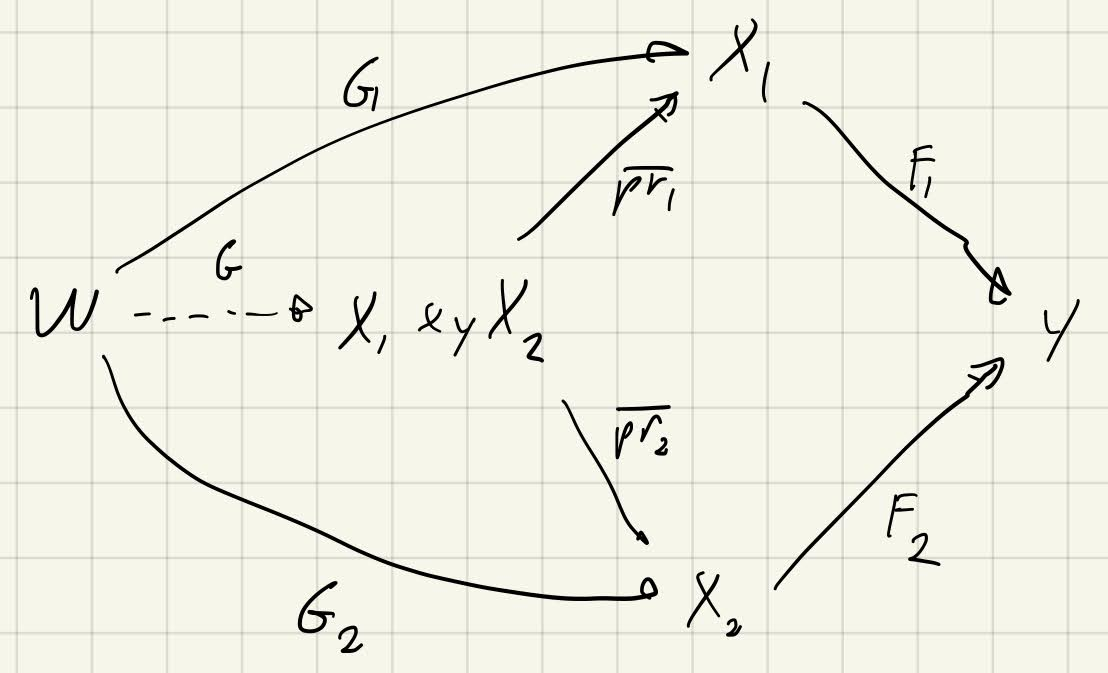
\includegraphics[width=8cm]{res/DG/DG12_universal_property.jpg}
  \label{figure: DG12_universal_property.jpg}
\end{figure}

\begin{proof}
  This being a more category-theory angle, and not being the focus here, we
  don't give a very detailed proof.
  \begin{itemize}
    \item Let $\iota : X_1 \times_Y X_2 \to X_1 \times X_2$ be the inclusion,
      then $\overline{\text{pr}}_i = \text{pr}_i \circ \iota$, which is smooth.
      Since we're using the fibre product, we then get $F_1 \circ
      \overline{\text{pr}}_1 = F_2 \circ \overline{\text{pr}}_2$ as required.
    \item Using the fact that post composition with $\iota$ gives a bijection
      between smooth maps from maps $W \to X_1 \times_Y X_2$ to maps $W \to X_1
      \times X_2$ with image $X_1 \times_Y X_2$ provides a proof. The details
      are left as an exercise (unfortunately). [End of DG 12]
  \end{itemize}
\end{proof}

\subsection{Manifolds with Boundaries}

All the manifolds we've dealt with so far all had to be more or less open sets,
so how do we generalise all our notions to manifolds that might be partially
closed sets, or have non-empty boundaries?

\begin{definition}
A \textbf{topological $n$-manifold with boundary} is a Hausdorff,
second-countable topological space $X$ such that for every point $p \in X$ we
can find an open set $U \ni p$, and (new) also a set $V$ open in either
$\mathbb{R}^n$ or $\mathbb{R}_{\geq 0} \times \mathbb{R}^{n - 1}$ together with
homeomorphism $\phi : U \to V$. Here points where $V$ can be picked to be an open
set in $\mathbb{R}^n$ are called the \textbf{interior} of $X$, denoted
$\mathring{X}$ , and points where $V$ must be a subset of $\mathbb{R}_{\geq 0}
\times \mathbb{R}^{n - 1}$ are called part of the boundary, denoted $\partial X$.
\end{definition}

One can use algebraic topology (use contractibility) to show that the boundary
and interior are well-defined. Also, note that $\mathbb{R}^n$ is embedded in
$\mathbb{R}_{\geq 0} \times \mathbb{R}^{n - 1}$ so really it is not necessary to
consider the possibility that $V$ lies in $\mathbb{R}^n$. Nevertheless, it is
convenint to think of things this way, and that is generally how we split
between the interior and the boundary, even though it is not strictly necessary.

Now, do we run into any problems generalising all the notions we had previously
come up with to these manifolds with boundaries? In fact, surprisingly little
changes. The only modification has to be made is that

\begin{definition}
A map $F : W \to \mathbb{R}^m$ for manifold with boundary $W \subseteq
\mathbb{R}_{\geq 0} \times \mathbb{R}^n$ is \textbf{smooth}
if there exists open $W' \subseteq \mathbb{R}^n$ such that $W' \supseteq W$ and
extension $\bar{F}$ of $F$ to $W'$ that is smooth as a map from $W' \to
\mathbb{R}^m$. 
\end{definition}

For the rest, we can easily transfer all definitions, including the notion of a
smooth $n$-manifold with boundary as just adding a smooth structure as before.
This notion also is highly compatible with our original notion in the sense that
if the boundary is empty we simply recover our original manifold. Now, we just
have the advantage that we can consider space such as $[0, 1]$ to be a manifold
with boundary with interior (always a normal manifold) $(0, 1)$ and boundary
$\{0, 1\}$.

\begin{proposition}
If $X$ is an $n$-manifold with boundary then $\mathring{X}$ is a $n$-manifold,
and $\partial X$ is an $(n - 1)$-manifold.
\end{proposition}
\begin{proof}
  It is obvious for the interior, just by transferring charts. For the boundary,
  take a point $p \in \partial X$, then there exists $\phi : U \to V \subseteq
  \mathbb{R}_{\geq 0} \times \mathbb{R}^{n - 1}$, so restricting to $\partial U
  = \phi^{-1}(V \cap (\{0\} \times \mathbb{R}^{n - 1}))$ an open neighbourhood
  of $p \in \partial X$. $\phi$ restricted to $\partial U$ forms a chart, and
  together these form the required smooth structure on $\partial X$.
\end{proof}

\begin{example}
  If $X$ is a manifold with boundary and $Y$ is an ordinary manifold, then $X
  \times Y$ is a manifold with boundary with interior $\mathring{X} \times Y$
  and boundary $\partial X \times Y$.
\end{example}

\begin{example}
  If both $X, Y$ are manifolds with boundaries, then $X \times Y$ may not be a
  manifold with boundary. THe chief example is with $[0, 1]^2$ the corners fail
  to be part of the $boundary$ as we defined it, sicne they are two dimensions
  lower, not just one dimension lower than the interior of the manifold. There
  exists a good theory of such manifolds, but they are not described in this
  course.
\end{example}

\begin{example}
All 1-manifolds with boundary that are also connected are up to diffeomorphism:
$(0, 1), [0, 1], [0, 1), $ and $S^1$. To justify this, Hausdorff and
second-countability are very important. 
\end{example}

Perhaps one other definition needs a bit of modifying:

\begin{definition}
  A smooth map $F : W \to X$ is \textbf{transverse} to $Z$ if $F|_{\mathring{X}}
  \pitchfork Z$ and $F|_{\partial W} \pitchfork Z$.
\end{definition}

\begin{proposition}
  If $F \pitchfork Z$ then $F^{-1}(Z)$ is a manifold with boundary of
  dimension $\text{dim}(W) - \text{codim}(Z)$. Moreover,
  $$ \partial F^{-1}(Z) = F^{-1}(Z) \cap \partial W $$
\end{proposition}

The proof of this is left as an exercise. An example of this that will be useful
later on is:

\begin{example}
  If $F_0, F_1$ are homotopic with homotopy $F: [0, 1] \times W \to X$ then if
  $F \pitchfork Z \subseteq X$ then $F^{-1}(Z)$ is a manifold with boundary with
  $$ \partial(F^{-1}(Z)) = F_0^{-1}(Z) \coprod F_1^{-1}(Z) $$
  [End of DG 13]
\end{example}

\subsection{Intersection Theory}

Now that we've set up the basics of our theory, we look at some of the
consequences it has, most notably in topology. In this (sub)section we will
assume that $X$ is an $n$-manifold, $Z$ is a submanifold of codimension $k$ that
is closed as a set in $X$, and $W$ is a compact $k$-manifold.

Notice that $Z$ is closed in $X$ iff the inclusion of $Z$
in $X$ is \textbf{proper} (pre-images of compact sets are compact), so such submanifolds
are somtimes called \textbf{properly embedded}.

Also, notice that $Z$ being closed and a submanifold of $X$ is equivalent to the
statement $\forall p \in X$ (not just $Z$ this time) $\exists$ local coordinates
$X$ on an open set $U \ni p$ such that $Z$ is given by $x_1 = \dots = x_k = 0$.

Finally, just in terms of terminology, a manifold is sometimes called
$\textbf{closed}$ if it is compact without boundary, but this is a strictly
stronger statement than it being closed in the set sense. That's why the term
properly embedded is sometimes preferred to describe the situation we have here
(or just closed as sets).

Now the key point throughout this
lecture, and the reason we require compactness and closedness is that if we take
take $\iota_0 : W \to X$ to be transverse to $Z$, then $Z \cap \iota_0 (W)$ is a
0-manifold (since the dimension are the same), and $Z$ closed in $X$ means this
intersection is a closed subspace of compact space $\iota_0(W)$, meaning that $Z
\cap \iota_0(W)$ is a finite collection of points. In particular, we can imagine
the following here:

\begin{figure}[H]
  \centering
  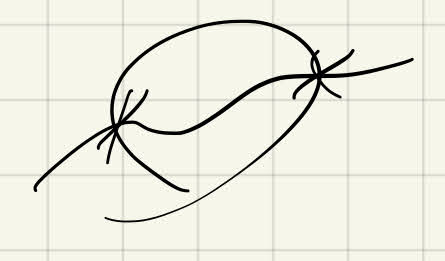
\includegraphics[width=5cm]{res/DG/DG14_intersecting_spaces.jpg}
  \caption{Intersecting Spaces}
  \label{DG14_interesecting_spaces.jpg}
\end{figure}

Even more amazingly, for any homotopy moving $\iota$ around, $\iota$ can only
fail to be transverse in two ways: either two points collide and disappear, or
they are born in pairs.

\begin{figure}[H]
  \centering
  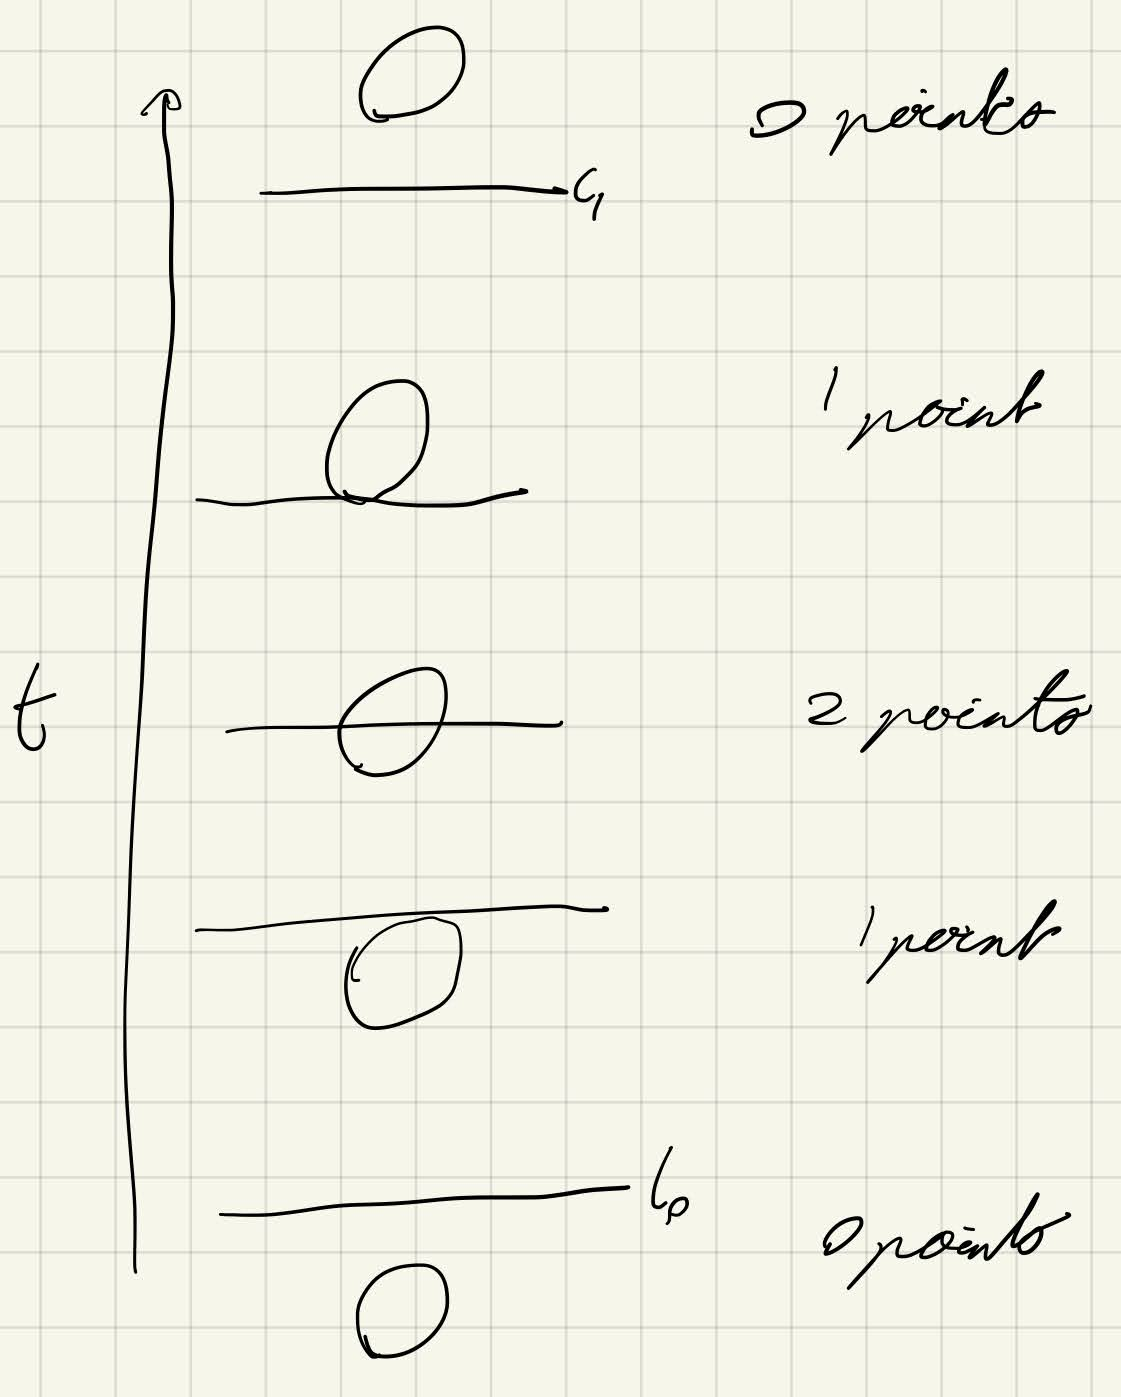
\includegraphics[width=6cm]{res/DG/DG14_moving_line.jpg}
  \label{DG14_moving_line.jpg}
\end{figure}

Consequently, we can argue that for any $N_f = N_i + 2(\text{births - deaths})$.
Generalising this to non-inclusions (really all we need is a smooth map), we
find that for any two smooth $F_0, F_1 : W \to X$ transverse to $X$, and we
assume there exists a homotopy between them, the

\begin{theorem}
  $F_0^{-1}(Z), F_1^{-1}(Z)$ have the same cardinality mod 2.
\end{theorem}

\begin{proof}
We justify this by assuming that for any homotopy $F$ we can find a small
pertubiation so that $F_t$ is always transverse to $Z.$ Then $F \pitchfork Z$
and $F^{-1}(Z)$ us compact (it forms a manifold with boundary containing $r$
copies of $[0, 1]$, and $s$ copies of $S^1$). Because of that when counting we
find that

$$ 2r = |\partial F^{-1}(Z)| = |F_0^{-1}(Z)| + |F_1^{-1}(Z)| $$

which gives our result.
\end{proof}

This is of huge value in topology. Examples include showing that the rings $\{0\}
\times S^1$ and $S^1 \times \{0\}$ are not homotopic since if $Z$ is one of
these loops, and $F(W)$ is the other loop, then if we could make $F$ homotopic
to something projecting onto $Z$ we'd be moving something with exactly one
intersection with $Z$ ($F(W)$) to something with 0 such intersections (a small
pertubation of $Z$ with itself is disjoint).

Perhaps a better example is that with some work one can show that $SO(3)$ is not
simply connected. The specific example used here is that if $Z$ is a submanifold
containing all rotations by $\pi$, then by identifying the axis of rotation with
a point in $\mathbb{RP}^2$ we see that these spaces are diffeomorphic. Then if
we consider any axis $l$, and $\gamma : S^1 \to SO(3)$ mapping $e^{i\theta}
\mapsto $ a rotation about $l$ by $\theta$ then $\gamma \pitchfork Z$, and they
intersect exactly at one point (when $\theta = \pi$). This means the space is
not simply connected since then it would be homotopic to the constant map which
has only 1 point of intersection.

Now, in the particular case that $k=n$, so both $W$, and $X$ are $n$-manifolds,
but $W$ is compact, then for any regular value $p \in X$ of $F : W \to X$ we can
compute $|F^{-1}(p)|$. If $X$ is connected, this is independent of $p$, and we
call this the \textbf{degree} of $F$. This is related to the winding number, and
refers to how frequently we ``repeat'' $W$ in $X$. Here is a proof of invariance
with respect to the point chosen

\begin{proof}
  If $\tilde{F}_p : W \to X \times X, w \mapsto (F(w), p) $ (and we have
  similarly $\tilde{F}_q$), then if $\Delta$ is the diagonal on the space.
  Connectivity means path connectivity on a smooth manifold, meaning that we can
  find a path $\gamma$ connecting $p$ and $q.$ We can then (exercise) construct
  a homotopy between the two $\tilde{F}$s, giving us the same degree mod 2.
\end{proof}

\begin{theorem}
The degree of $F$ is invariant under homotopies.
\end{theorem}

This follows from the results we've been considering.

Some examples include that the identity map has degree 1, while a constant map
has degree 0, meaning in particular that the identity map is not nullhomotopic
(an otherwise hard result!). Another more complex example is the following:

\begin{example}
There exists a degree 1 map from $T^2$ (the torus) to $S^2$, but not the other
way around. Constructing a map that does so is not too hard. Consider open
subset $U \subseteq T^2$, and treat $S^2 \equiv \mathbb{C] \cup \{\infty\}}$ and
send $U$ to $\mathbb{C}$, and the rest of the set to $\{\infty\}$. This has
degree one.

Showing that there is no map that does the same the other way around is harder,
but assume one does exist, and let $Z_1 = S^1 \times \{1\}, Z_2 = \{1\} \times
S^1$, then we see by homotopies that we can assume $F$ is transverse to $Z_1,
Z_2, Z_1 \cap Z_2$, so $F^{-1}(Z_i)$ are compact submanifolds of $S^2$ of
codimension 1. But in $T^2$ these meet at only one point, whereas in $S^2$ they
cross two times...
\end{example}

\begin{figure}[H]
\centering
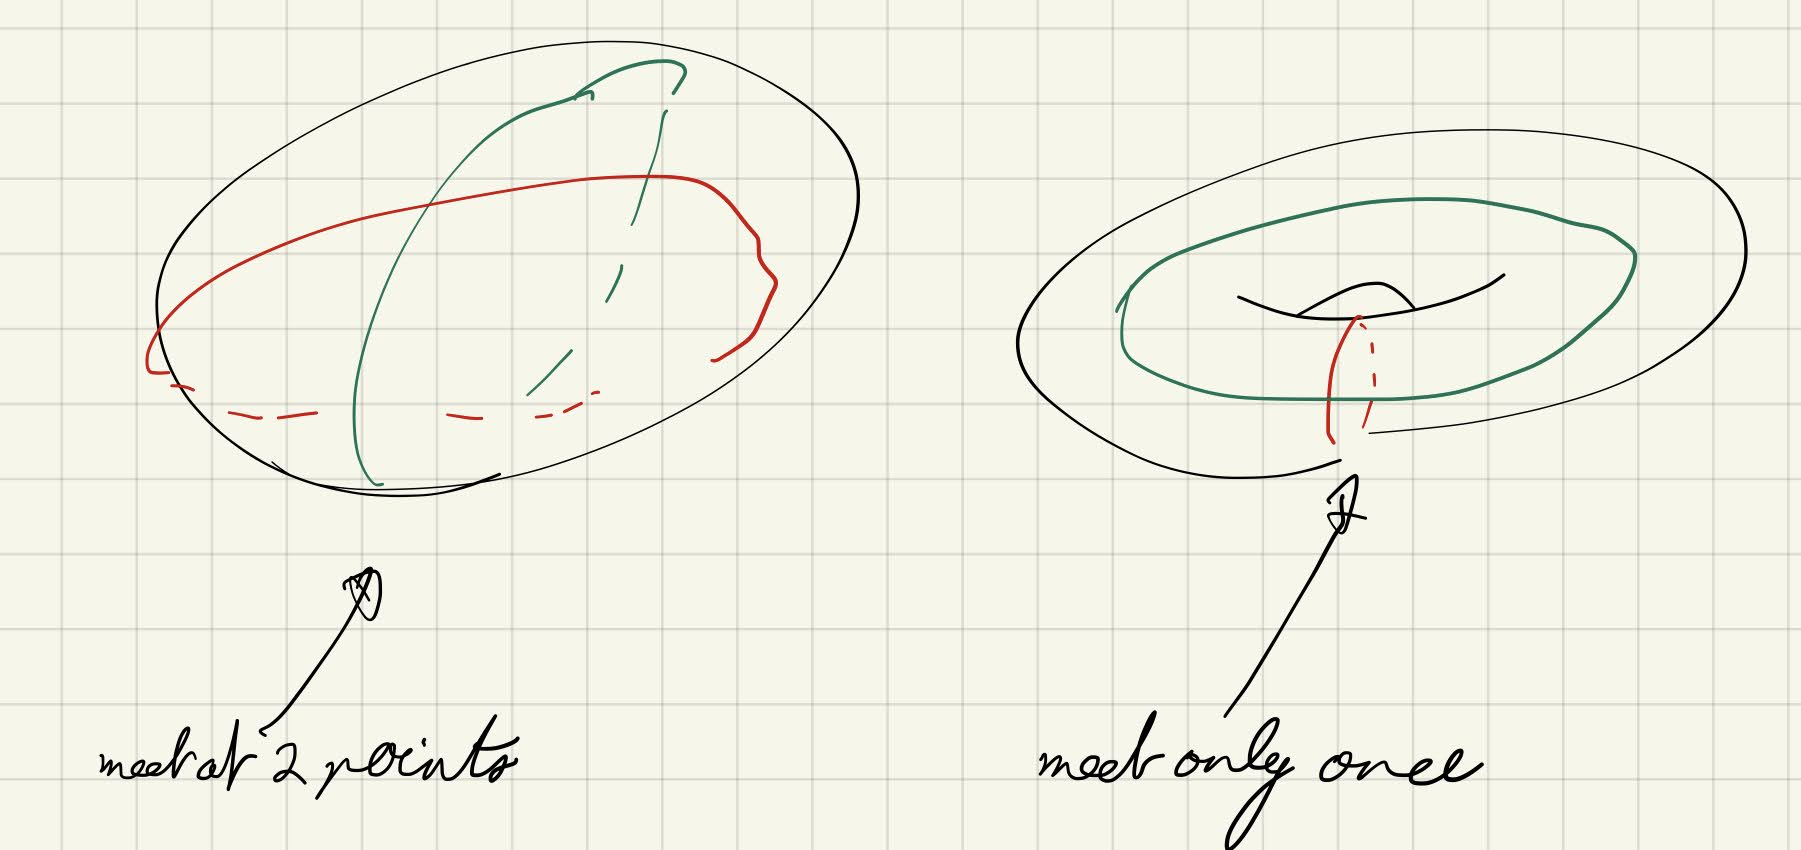
\includegraphics[width=10cm]{res/DG/DG14_torus_sphere.jpg}
\end{figure}

This is related to cup products in algebraic topology.

Now we can generalise our theorem a bit. Firstly, if we are working on an
orientable surface we can upgrade from working on $\mathbb{Z} / 2$ to working on
$\mathbb{Z}$ which is a significant improvement. Secondly, instead of working
with homotopy equivalenec, we actually only need maps to have a \textbf{cobordism}. That
is we only need a map $F : W \to X$ on a manifold with boundary $W$ such that
the boundary on $W$ corresponds to $W_0, W_1$ the domains of $F_0, F_1$, and of
course it is smooth. The internal structure of $W$ might be very complicated
though. Here, the cobordism $[0, 1] \times W$ is called the \textbf{trivial
  cobodrism} which corresponds to the cobordism used for homotopies.

To include orientation, we actually need maps to be \textbf{orient-cobordant}
meaning that the boundary of the cobodrism satisfies $\partial Y = -W_0 \coprod
W_1$. Once we get this we can state the full version of our new theorem:

\begin{theorem}
  If $F_0, F_1$ are cobordant then $\#F_0^{-1}(Z) = \#F_1^{-1}(Z)$ on orientable manifolds.
\end{theorem}

This is quite remarkable, but unfortunately the details are not proven here.
[End of DG14]

\end{document}
